\documentclass{standalone}
\usepackage{tikz}
\usetikzlibrary{patterns, positioning}
\usepackage[sfdefault]{ClearSans} %% option 'sfdefault' activates Clear Sans as the default text font
\usepackage[T1]{fontenc}

\begin{document}
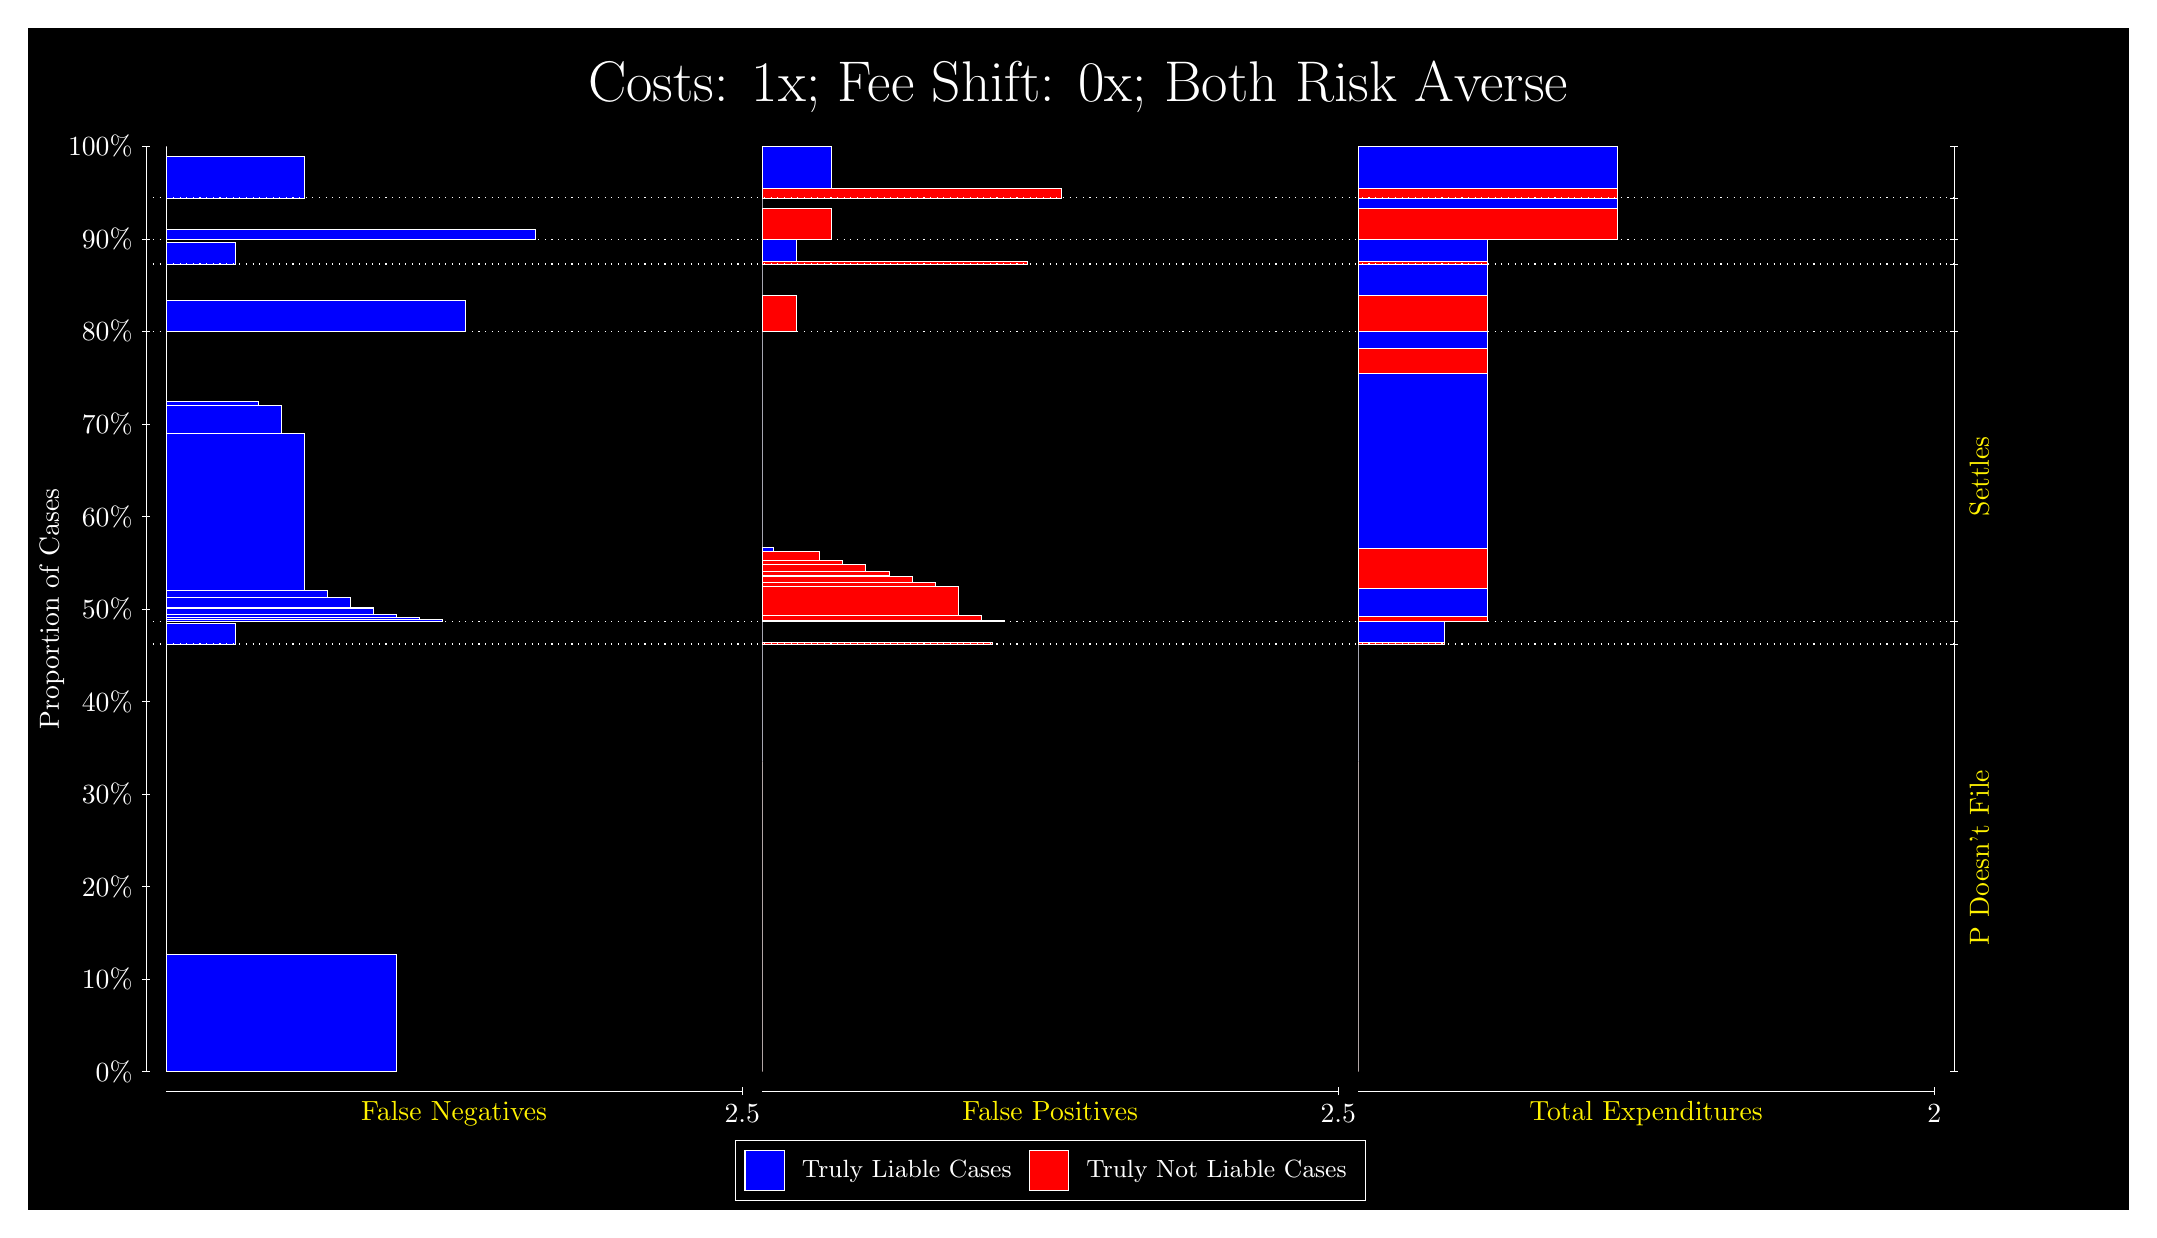
\begin{tikzpicture}
\draw[fill=black] (0,0) rectangle (26.667,15);
\draw[text=white] (0,13.5) rectangle (26.667,15) node[midway] {\huge Costs: 1x; Fee Shift: 0x; Both Risk Averse};
\draw[white, very thin] (1.5,1.75) -- (1.5,13.5);
\node[rotate=90, text=white, anchor=center] at (0.3, 7.625) {Proportion of Cases};
\draw[white, very thin] (1.45,1.75) -- (1.55,1.75);
\node[text=white, anchor=east] at (1.45, 1.75) {0\%};
\draw[white, very thin] (1.45,2.925) -- (1.55,2.925);
\node[text=white, anchor=east] at (1.45, 2.925) {10\%};
\draw[white, very thin] (1.45,4.1) -- (1.55,4.1);
\node[text=white, anchor=east] at (1.45, 4.1) {20\%};
\draw[white, very thin] (1.45,5.275) -- (1.55,5.275);
\node[text=white, anchor=east] at (1.45, 5.275) {30\%};
\draw[white, very thin] (1.45,6.45) -- (1.55,6.45);
\node[text=white, anchor=east] at (1.45, 6.45) {40\%};
\draw[white, very thin] (1.45,7.625) -- (1.55,7.625);
\node[text=white, anchor=east] at (1.45, 7.625) {50\%};
\draw[white, very thin] (1.45,8.8) -- (1.55,8.8);
\node[text=white, anchor=east] at (1.45, 8.8) {60\%};
\draw[white, very thin] (1.45,9.975) -- (1.55,9.975);
\node[text=white, anchor=east] at (1.45, 9.975) {70\%};
\draw[white, very thin] (1.45,11.15) -- (1.55,11.15);
\node[text=white, anchor=east] at (1.45, 11.15) {80\%};
\draw[white, very thin] (1.45,12.325) -- (1.55,12.325);
\node[text=white, anchor=east] at (1.45, 12.325) {90\%};
\draw[white, very thin] (1.45,13.5) -- (1.55,13.5);
\node[text=white, anchor=east] at (1.45, 13.5) {100\%};

\draw[white, very thin] (24.457,1.75) -- (24.457,13.5);
\draw[white, very thin] (24.407,1.75) -- (24.507,1.75);
\node[anchor=west] at (24.407, 1.75) {};
\draw[white, very thin] (24.407,7.179) -- (24.507,7.179);
\node[anchor=west] at (24.407, 7.179) {};
\draw[white, very thin] (24.407,7.4696) -- (24.507,7.4696);
\node[anchor=west] at (24.407, 7.4696) {};
\draw[white, very thin] (24.407,11.152) -- (24.507,11.152);
\node[anchor=west] at (24.407, 11.152) {};
\draw[white, very thin] (24.407,12.006) -- (24.507,12.006);
\node[anchor=west] at (24.407, 12.006) {};
\draw[white, very thin] (24.407,12.315) -- (24.507,12.315);
\node[anchor=west] at (24.407, 12.315) {};
\draw[white, very thin] (24.407,12.845) -- (24.507,12.845);
\node[anchor=west] at (24.407, 12.845) {};
\draw[white, very thin] (24.407,13.5) -- (24.507,13.5);
\node[anchor=west] at (24.407, 13.5) {};

\draw[white, very thin, fill=blue] (1.75,1.75) rectangle (4.6775,3.2391);
\draw[white, very thin, fill=red] (1.75,3.2391) rectangle (1.75,7.179);
\draw[white, very thin, fill=blue] (1.75,7.179) rectangle (2.6283,7.4445);
\draw[white, very thin, fill=red] (1.75,7.4445) rectangle (1.75,7.4696);
\draw[white, very thin, fill=blue] (1.75,7.4696) rectangle (5.2631,7.4977);
\draw[white, very thin, fill=blue] (1.75,7.4977) rectangle (4.9703,7.5183);
\draw[white, very thin, fill=blue] (1.75,7.5183) rectangle (4.6775,7.5535);
\draw[white, very thin, fill=blue] (1.75,7.5535) rectangle (4.3848,7.6351);
\draw[white, very thin, fill=blue] (1.75,7.6351) rectangle (4.3848,7.6449);
\draw[white, very thin, fill=blue] (1.75,7.6449) rectangle (4.092,7.768);
\draw[white, very thin, fill=blue] (1.75,7.768) rectangle (3.7993,7.8584);
\draw[white, very thin, fill=blue] (1.75,7.8584) rectangle (3.5065,9.8511);
\draw[white, very thin, fill=blue] (1.75,9.8511) rectangle (3.2138,10.21);
\draw[white, very thin, fill=blue] (1.75,10.21) rectangle (2.921,10.264);
\draw[white, very thin, fill=red] (1.75,10.264) rectangle (1.75,11.152);
\draw[white, very thin, fill=blue] (1.75,11.152) rectangle (5.5558,11.551);
\draw[white, very thin, fill=red] (1.75,11.551) rectangle (1.75,12.006);
\draw[white, very thin, fill=blue] (1.75,12.006) rectangle (2.6283,12.278);
\draw[white, very thin, fill=red] (1.75,12.278) rectangle (1.75,12.315);
\draw[white, very thin, fill=blue] (1.75,12.315) rectangle (6.4341,12.442);
\draw[white, very thin, fill=red] (1.75,12.442) rectangle (1.75,12.845);
\draw[white, very thin, fill=blue] (1.75,12.845) rectangle (3.5065,13.373);
\draw[white, very thin, fill=red] (1.75,13.373) rectangle (1.75,13.5);
\draw[white, very thin, fill=red] (9.3189,1.75) rectangle (9.3189,5.6899);
\draw[white, very thin, fill=blue] (9.3189,5.6899) rectangle (9.3189,7.179);
\draw[white, very thin, fill=red] (9.3189,7.179) rectangle (12.246,7.2041);
\draw[white, very thin, fill=blue] (9.3189,7.2041) rectangle (9.3189,7.4696);
\draw[white, very thin, fill=red] (9.3189,7.4696) rectangle (12.393,7.4817);
\draw[white, very thin, fill=red] (9.3189,7.4817) rectangle (12.1,7.542);
\draw[white, very thin, fill=red] (9.3189,7.542) rectangle (11.807,7.9084);
\draw[white, very thin, fill=red] (9.3189,7.9084) rectangle (11.515,7.9624);
\draw[white, very thin, fill=red] (9.3189,7.9624) rectangle (11.222,8.0447);
\draw[white, very thin, fill=red] (9.3189,8.0447) rectangle (10.929,8.0525);
\draw[white, very thin, fill=red] (9.3189,8.0525) rectangle (10.929,8.1023);
\draw[white, very thin, fill=red] (9.3189,8.1023) rectangle (10.636,8.1888);
\draw[white, very thin, fill=red] (9.3189,8.1888) rectangle (10.344,8.2426);
\draw[white, very thin, fill=red] (9.3189,8.2426) rectangle (10.051,8.3575);
\draw[white, very thin, fill=blue] (9.3189,8.3575) rectangle (9.4652,8.411);
\draw[white, very thin, fill=blue] (9.3189,8.411) rectangle (9.3189,11.152);
\draw[white, very thin, fill=red] (9.3189,11.152) rectangle (9.758,11.606);
\draw[white, very thin, fill=blue] (9.3189,11.606) rectangle (9.3189,12.006);
\draw[white, very thin, fill=red] (9.3189,12.006) rectangle (12.686,12.043);
\draw[white, very thin, fill=blue] (9.3189,12.043) rectangle (9.758,12.315);
\draw[white, very thin, fill=red] (9.3189,12.315) rectangle (10.197,12.718);
\draw[white, very thin, fill=blue] (9.3189,12.718) rectangle (9.3189,12.845);
\draw[white, very thin, fill=red] (9.3189,12.845) rectangle (13.125,12.972);
\draw[white, very thin, fill=blue] (9.3189,12.972) rectangle (10.197,13.5);
\draw[white, very thin, fill=red] (16.888,1.75) rectangle (16.888,5.6899);
\draw[white, very thin, fill=blue] (16.888,5.6899) rectangle (16.888,7.179);
\draw[white, very thin, fill=red] (16.888,7.179) rectangle (17.986,7.2041);
\draw[white, very thin, fill=blue] (16.888,7.2041) rectangle (17.986,7.4696);
\draw[white, very thin, fill=red] (16.888,7.4696) rectangle (18.534,7.5299);
\draw[white, very thin, fill=blue] (16.888,7.5299) rectangle (18.534,7.8893);
\draw[white, very thin, fill=red] (16.888,7.8893) rectangle (18.534,8.3998);
\draw[white, very thin, fill=blue] (16.888,8.3998) rectangle (18.534,10.616);
\draw[white, very thin, fill=red] (16.888,10.616) rectangle (18.534,10.933);
\draw[white, very thin, fill=blue] (16.888,10.933) rectangle (18.534,11.152);
\draw[white, very thin, fill=red] (16.888,11.152) rectangle (18.534,11.606);
\draw[white, very thin, fill=blue] (16.888,11.606) rectangle (18.534,12.006);
\draw[white, very thin, fill=red] (16.888,12.006) rectangle (18.534,12.043);
\draw[white, very thin, fill=blue] (16.888,12.043) rectangle (18.534,12.315);
\draw[white, very thin, fill=red] (16.888,12.315) rectangle (20.181,12.718);
\draw[white, very thin, fill=blue] (16.888,12.718) rectangle (20.181,12.845);
\draw[white, very thin, fill=red] (16.888,12.845) rectangle (20.181,12.972);
\draw[white, very thin, fill=blue] (16.888,12.972) rectangle (20.181,13.5);
\draw[white, dotted] (1.5,7.179) -- (24.457,7.179);
\draw[white, dotted] (1.5,7.4696) -- (24.457,7.4696);
\draw[white, dotted] (1.5,11.152) -- (24.457,11.152);
\draw[white, dotted] (1.5,12.006) -- (24.457,12.006);
\draw[white, dotted] (1.5,12.315) -- (24.457,12.315);
\draw[white, dotted] (1.5,12.845) -- (24.457,12.845);
\draw[white, very thin] (1.75,1.5) -- (9.0689,1.5);
\node[text=yellow, anchor=north] at (5.4094, 1.5) {False Negatives};
\draw[white, very thin] (9.0689,1.45) -- (9.0689,1.55);
\node[text=white, anchor=north] at (9.0689, 1.45) {2.5};

\draw[white, very thin] (9.3189,1.5) -- (16.638,1.5);
\node[text=yellow, anchor=north] at (12.978, 1.5) {False Positives};
\draw[white, very thin] (16.638,1.45) -- (16.638,1.55);
\node[text=white, anchor=north] at (16.638, 1.45) {2.5};

\draw[white, very thin] (16.888,1.5) -- (24.207,1.5);
\node[text=yellow, anchor=north] at (20.547, 1.5) {Total Expenditures};
\draw[white, very thin] (24.207,1.45) -- (24.207,1.55);
\node[text=white, anchor=north] at (24.207, 1.45) {2};

\node[text=yellow, centered, rotate=90] at (24.777, 4.4645) {P Doesn't File};

\node[text=yellow, centered, rotate=90] at (24.777, 9.3107) {Settles};





\draw (12.978300999999998,1.5) node[draw=none] (baseCoordinate) {};
\begin{scope}[align=center]
        \matrix[scale=0.5, draw=white, below=0.5cm of baseCoordinate, nodes={draw}, column sep=0.1cm]{
            \node[rectangle, draw, minimum width=0.5cm, minimum height=0.5cm, fill=blue] {}; &
            \node[draw=none, font=\small, text=white] (B) {Truly Liable Cases}; &
            \node[rectangle, draw, minimum width=0.5cm, minimum height=0.5cm, fill=red] {}; &
            \node[draw=none, font=\small, text=white] (B) {Truly Not Liable Cases}; \\
            };
\end{scope}

\end{tikzpicture}
\end{document}